\chapter{Appendix}

\section{Supplementary Figures and Tables}

\begin{table}[htbp]
    \centering
    \includegraphics[width=\textwidth]{tables/rq-b.pdf}
    \shortcaption{Extended evaluation results for OpenCoder-1.5B-Base}{Extended table presenting the evaluation results for OpenCoder-1.5B-Base, which underwent the repository-level pre-training stage. A more detailed description of the evaluation setup is provided in \sectionref{sec:evaluation}.}\label{tab:ocoder-extension-extended}
\end{table}

\begin{table}[htbp]
    \centering
    \includegraphics[width=\textwidth]{tables/rq-a2-gradient-masking.pdf}
    \shortcaption{Evaluation of DeepSeek-Coder-Base 1.3B fine-tuned with and without gradient masking}{Exact Match scores for DeepSeek-Coder-Base 1.3B fine-tuned on composers generating inlier repository context for the completion file under two training setups: with and without gradient masking}\label{tab:dseek-gradient-masking}
\end{table}

\begin{table}[htbp]
    \centering
    \includegraphics[width=\textwidth]{tables/rq-b-gradient-masking.pdf}
    \shortcaption{Evaluation of repository-level pre-trained OpenCoder-1.5B-Base with and without gradient masking}{Exact Match scores for repository-level pre-trained OpenCoder-1.5B-Base on composers generating inlier repository context for the completion file under two training setups: with and without gradient masking}\label{tab:ocoder-gradient-masking}
\end{table}

\begin{figure}[ht]
    \centering
    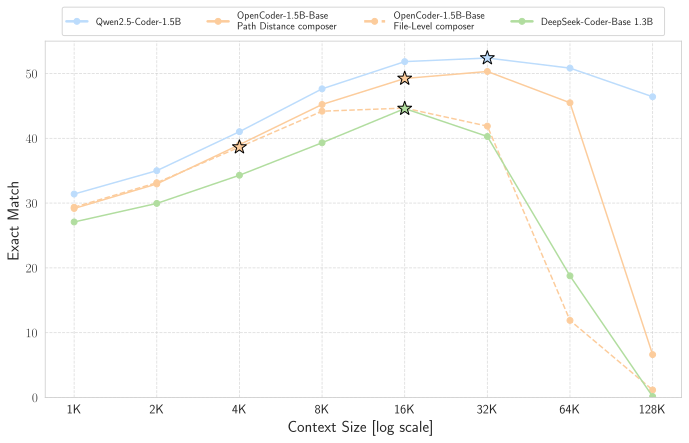
\includegraphics[width=\textwidth]{figures/beyond-training-window-infile.pdf}
    \shortcaption{Performance scaling beyond context extension window (\textit{infile})}{Evaluation of the performance scaling beyond the context extension window. The \textit{infile} line type from the LCA benchmark is selected for visualization; the corresponding \figureref{fig:beyond-training-window-inproject} presents results for the \textit{inproject} category. ``1K'' refers to 1,024 tokens. The \raisebox{-0.3ex}{\FiveStarOpen} markers denote the context length used during repository-level pre-training stage.}\label{fig:beyond-training-window-infile}
\end{figure}
